\documentclass{article}
\usepackage[utf8]{inputenc}

\title{Eye-tracking for Head Mounted Devices}
\author{Dr. Uri Wollner, Soliman Nasser, Nadav Yehonatan Arbel}
\date{December 2018}

\usepackage{natbib}
\usepackage{graphicx}
\usepackage{enumitem}
\usepackage{multirow}
\usepackage[dvipsnames]{xcolor}
\usepackage[legalpaper, margin=1.5in]{geometry}
\usepackage{amsmath, algorithmic, algorithm}
%\usepackage[]{algorithm2e}
\begin{document}

\maketitle

\section{Introduction}

The eyes play an important role in the perception of our surrounding as well as in communication with other human beings. Our eyes' gaze direction, as estimated by others, indicate what are we interested in or focus our attention on. Apart from the behavioral aspect, estimating gaze direction also plays a role in Mixed Reality, AI assistant devices, automotive, panel control, Human-Robot interaction, users authentication and many other applications. 

In practice, estimating human gaze directions through remote sensing methods, such as cameras, is still a challenge \cite{HansenJi2010}. Methods that are based on active illumination and infrared imaging typically require localization of glints generated on the surface of the cornea to estimate gaze direction. One issue with this approach is that when the cornea's location w.r.t to the imaging device does not produce visible glints, the algorithm cannot estimate the gaze direction of the user. Therefore, it is desirable to design a glint-free eye-tracking method.

Several glint-free eye-tracking methods have been proposed in the past. In particular, \cite{SwirskiDodgson2013} developed a temporal model-based approach in which a 3D eye model is fitted to a series of pupil contours extracted from images recorded with a single near-eye camera.  \cite{LuEtAl2016} proposed a similar method to \cite{SwirskiDodgson2013} but instead of fitting an eye model to pupil contours, they fitted an eye model to extracted limbus contours. Both  \cite{SwirskiDodgson2013} and \cite{LuEtAl2016} rely on the assumption that the center of rotation of the eyeball is fixed in the eye camera coordinate system.

One challenge of such contour-based methods is, firstly, locating the relevant contours for gaze estimation.  Another challenge is the refraction of light rays at the cornea surface. The latter challenge is particularly important as \cite{VillanuevaCabeza2008} showed that ignoring cornea refraction will incur high gaze estimation errors, up to several degree. Gaze estimation methods that do account for cornea refraction include \cite{LaiEtAl2015} and \cite{dierkes18_etra}. \cite{LaiEtAl2015} proposed a contour-based method to provide a glint-free gaze estimation.  However, their setup required two eye cameras. In contrast, \cite{dierkes18_etra} proposed a single camera, glint-free, gaze estimation method but their eye model had multiple parameters that were considered constant. No attempt was made to optimize these eye parameters for single user.
 
Similar to other methods, Blink's robust gaze estimating solution for glasses equipped with IR/RGB camera is contour-based.  The technology is based on: (1) mathematical modelling of eye behavior and geometry, and (2) state-of-the-art computer-vision algorithms for pupil and iris detection.  In contrast to other studies, we present a more general model of the human eye, which includes an ellipsoidal cornea, refraction capabilities of the cornea, and optimization of eye parameters for a single user.  Our algorithm allows for automatic estimation of eyeball center of rotation. Thus, a user that has undergone a calibration process will not have to recalibrate the system due to glasses slippage or placement in different position.

\section{System setup}
\subsection{Overview}
To explore the feasibility and performance of Blink's A.EYE eye-tracking technology, we conducted a controlled experiment that included 10 subjects.  The experimental system comprised mainly of:
\begin{enumerate}
    \item Glasses frame
    \item Two IR cameras mounted on the glasses frame that monitor the left and right eye, respectively.
    \item Logitech camera mounted on the glasses frame, directed towards the world (e.g. world-camera).
    \item An LCD (55 Inch) display unit, on which we display several patterns (see Figure \ref{fig:pattern_monitor}) for the user to concentrate on during the experiment.
    \item A compute-unit on which the images from the camera are synchronized, stored and processed.
\end{enumerate}
The first three components comprised the Head Mounted Device (HMD).
%%%%%%%%%%%%%%%%%%%%%%%%%%%%%%%%%%%%%%%%%%%%%%%%%
\begin{figure}[h!]
    \center
    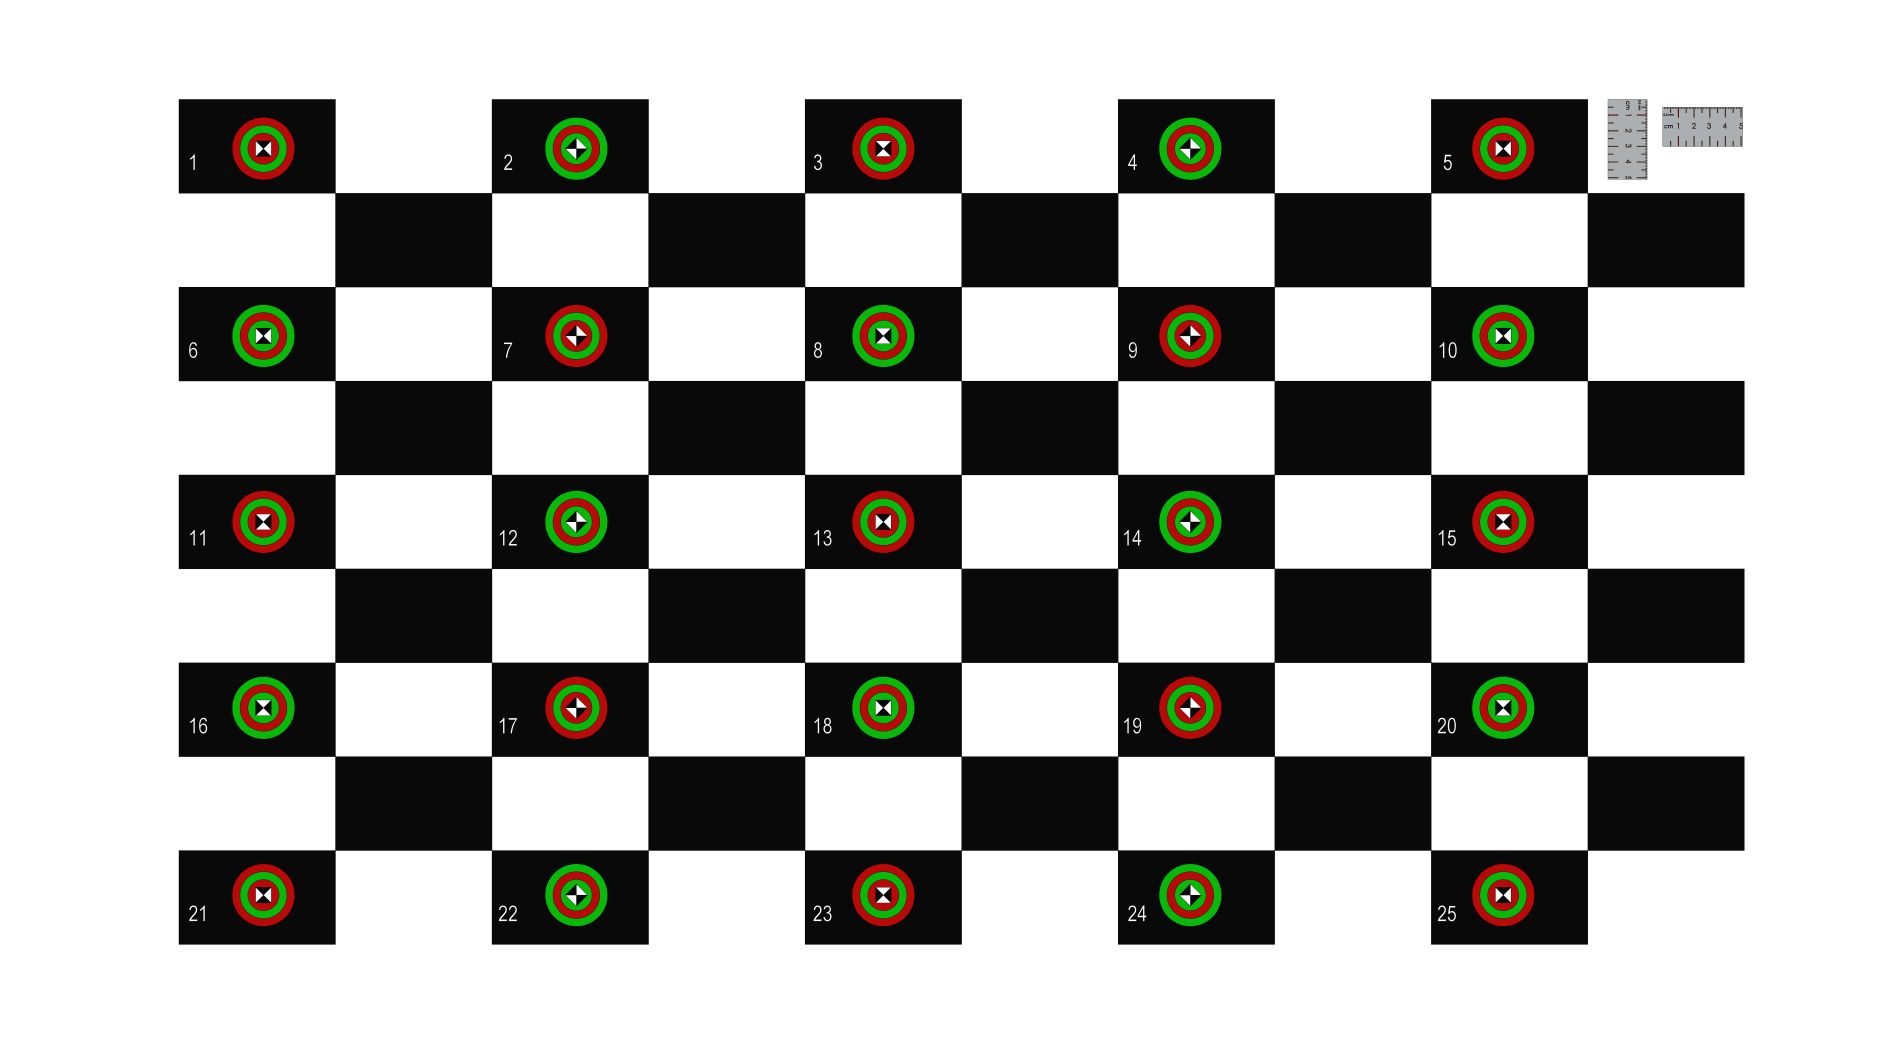
\includegraphics[scale=0.5]{./Pics/pattern_por}
    \caption{The display pattern as shown on the monitor.}
    \label{fig:pattern_monitor}
\end{figure}
%%%%%%%%%%%%%%%%%%%%%%%%%%%%%%%%%%%%%%%%%%%%%%%%%
\subsection{Coordinate Systems}
We have the following right-handed coordinate systems (CS) present in our experiment:
\begin{enumerate}[label=(\alph*)]
    \item \{ W; $x_w$, $y_w$, $z_w$\}, attached to the world camera;
    \item \{ M; $x_m$, $y_m$, $z_m$\}, attached to the monitor at the upper left corner of the monitor;
    \item \{ RC; $x_{rc}$, $y_{rc}$, $z_{rc}$\}, attached to the right eye camera;
    \item \{ LC; $x_{lc}$, $y_{lc}$, $z_{lc}$\}, attached to the left eye camera
\end{enumerate}

For the cameras CS (i.e. W, LR, and RC), the $z$ coordinate direction is defined along the normal to the image plane of each camera. The $x$ coordinate direction points along the horizontal direction as defined by the cameras' image plane.  The $z$ coordinate direction in the monitor CS is defined along the normal to the screen plane, while the $x$ coordinate direction points along the horizontal direction as defined by the screen plane.

\section{Video Streams}
Each subject was asked to wear the HMD and be seated in front and at the center of the display unit at a distance of 0.8 meters. The HMD's eye cameras were positioned such that the user’s left and right eyes were centered in the video frame.  The video data was recorded at a resolution of 400 $\times$ 400 pixels at a frame rate of 120 Hz. The subject was required to focus for 2 seconds on each of the markers displayed on the monitor.  During the 2 seconds time span, 120 frames from both eye cameras and the world camera were recorded.  The subject was required to limit the head movement throughout the experiment.  The data streams from the three HMD's cameras were synchronized with the pixel coordinates of the target points displayed on the monitor.

\section{Eye Camera Specifications}
As requested, we have used an infrared (IR) eye-camera with the following specifications. 

\begin{enumerate}
   \begin{itemize}
     \item Native resolution: 400x400 of monochrome channel with 120FPS (can obtain higher FPS with 200x200, 100x100 optional image size supported by ISP).
     \item Shutter Type: Global shutter.
     \item Package size: ~3x3 [mm] (sensor size of ~1x1[mm])
     \item Power consumption: Active mode: 85 mW @120 FPS. Standby mode: 15 $\mu$A.
   \end{itemize}
\end{enumerate}

It should be noted, that these parameters of packages size, resolution and power will be adjusted per the defined KPI's (camera location, FPS, etc.).      

\section{Cameras' extrinsic and intrinsic parameters}
All cameras used in this study were assumed to follow a pinhole camera model. The cameras relative and position relative to each other were fixed during the study.  The cameras' intrinsic as well as their distortion parameters were estimated using OpenCV's algorithm \cite{opencv_library}.  Specifically, a planar checkerboard pattern with known physical size was recorded by each of the cameras at several different view angles and distances.  These recorded images were then used as input to OpenCV's algorithm.

To compute the extrinsic relation between each of the cameras (i.e. homogeneous transformation matrices $\mathbf{H}$ between different camera coordinate systems), we performed the following procedure: 
\begin{enumerate}[label=(\alph*)]
    \item We placed the HMD in between three planar checkerboard patterns with known physical size. Two checkerboards were placed in front of the two eye camera, respectively. The additional checkerboard was placed in front of the world camera \textbf{(Figure XX)}. At this stage, we recorded the scene views of each of the cameras.
    \item Then, we repositioned only the HMD such that within the worlds' camera scene view all three checkerboard patterns are observed \textbf{(Figure XX)}.  At this stage, we recorded the scene view of the world camera.
\end{enumerate}

During step (a), the knowledge of the physical pattern observed by each camera, the cameras' intrinsic and distortion parameters, as well as OpenCV's algorithm, allowed us to estimate the translation ($\mathbf{t}$) and rotation ($\mathbf{R}$) of each checkerboard pattern w.r.t the camera's coordinate system. The purpose of step (b) was to obtain the position and orientation of each of the planar patterns relative to each other and, subsequently, compute $\mathbf{t}$ and $\mathbf{R}$ of each camera relative to the other two using the information from step (a).  That is, we estimated the $\mathbf{H}$s from the LC CS to W CS, defined by $\mathbf{H}^{LC}_{W}$, as well as from RC CS to W CS, defined by $\mathbf{H}^{RC}_{W}$.  Explicitly, $\mathbf{H}^1_2$ is defined as a $4 \times 4$ matrix which is comprised of rotation $\textbf{R}^1_2$ and translation $\textbf{t}^1_2$ components and it relates a point $[x_1, y_1, z_1]^T$ in one coordinate system to another $[x_2, y_2, z_2]^T$ through,
\begin{equation}
    \begin{bmatrix}
    x_2 \\
    y_2 \\
    z_2 \\
    1
  \end{bmatrix} = \mathbf{H}^1_2  \begin{bmatrix}
    x_1 \\
    y_1 \\
    z_1 \\
    1
  \end{bmatrix},
\end{equation}
where,
\begin{align*}
    \mathbf{H}^1_2 = \begin{bmatrix}
    \textbf{R}^1_2 & \textbf{t}^1_2\\
    \textbf{0} & 1
  \end{bmatrix} 
\end{align*}

To verify the validity of our transformation matrices \textbf{H}, we have...

\textcolor{red}{Soli: Can you please add the nice calibration setup images you have shown us. Also, the reprojected pattern from one camera viewpoint to another.}

\section{Gaze Estimation Framework}
The core of Blink's gaze estimation framework is based on a geometrical model of the eye constrained on 2D iris appearance in multiple eye images of the same user at the same recording session. The assumption in this approach is that the center of the rotation of the eye is stationary w.r.t the recording eye camera.  It should be emphasized that this approach does not require knowledge of the user's gaze direction.  The main requirement is that within the recorded frames there is sufficient variance in the position of the projected 2D iris.

\subsection{3D eye model}
The eye model is comprised of a sphere, representing the eyeball, as well as an ellipsoid, representing the cornea.  The specific parameters that are used to fully describe the eye model are noted in Table \ref{tab:model_parameters} and its geometrical representation is shown in Figure \ref{fig:model_drawing}. 

Our approach assumes the iris-sclera boundary (limbus) can be modelled as a circle, with radius $r_I$, lying on a plane that intersects a sphere. The sphere is used to model the eyeball. For simplicity, we assume that the eyeball's center of rotation ($ECR$) is located at the center of the sphere. This assumption is not a limiting factor of our model as we aim to estimate the $ECR$ of each user's eye and not specifically its eyeball center. 


%%%%%%%%%%%%%%%%%%%%%%%%%%%%%%%%%%%%%%%%%%%%%%%%%
\begin{table}[h!]
\caption{Spherical-eyeball-ellipsoidal-cornea model parameters}
\vspace{0.5cm}
\centering
\begin{tabular}{|l|c|c|c|c|c|c|c|c|c|c|}
\hline
Symbol & Meaning \\
\hline \hline
$ECR$ &  Eyeball center of rotation $(x,y,z)$\\ \hline 
$\bar{IC}$  &  Iris-Cornea offset\\ \hline
$\bar{IE}$ &  Iris-Eye-center offset \\ \hline
$r_I$ &  Iris radius \\ \hline
$r_C$ &  Cornea major axis radius \\ \hline
$\alpha, \beta$ &  Angular corrections to visual axis \\ 
\hline
\end{tabular}
\label{tab:model_parameters}
\end{table}
%%%%%%%%%%%%%%%%%%%%%%%%%%%%%%%%%%%%%%%%%%%%%%%%%
\begin{figure}[h!]
    \center
    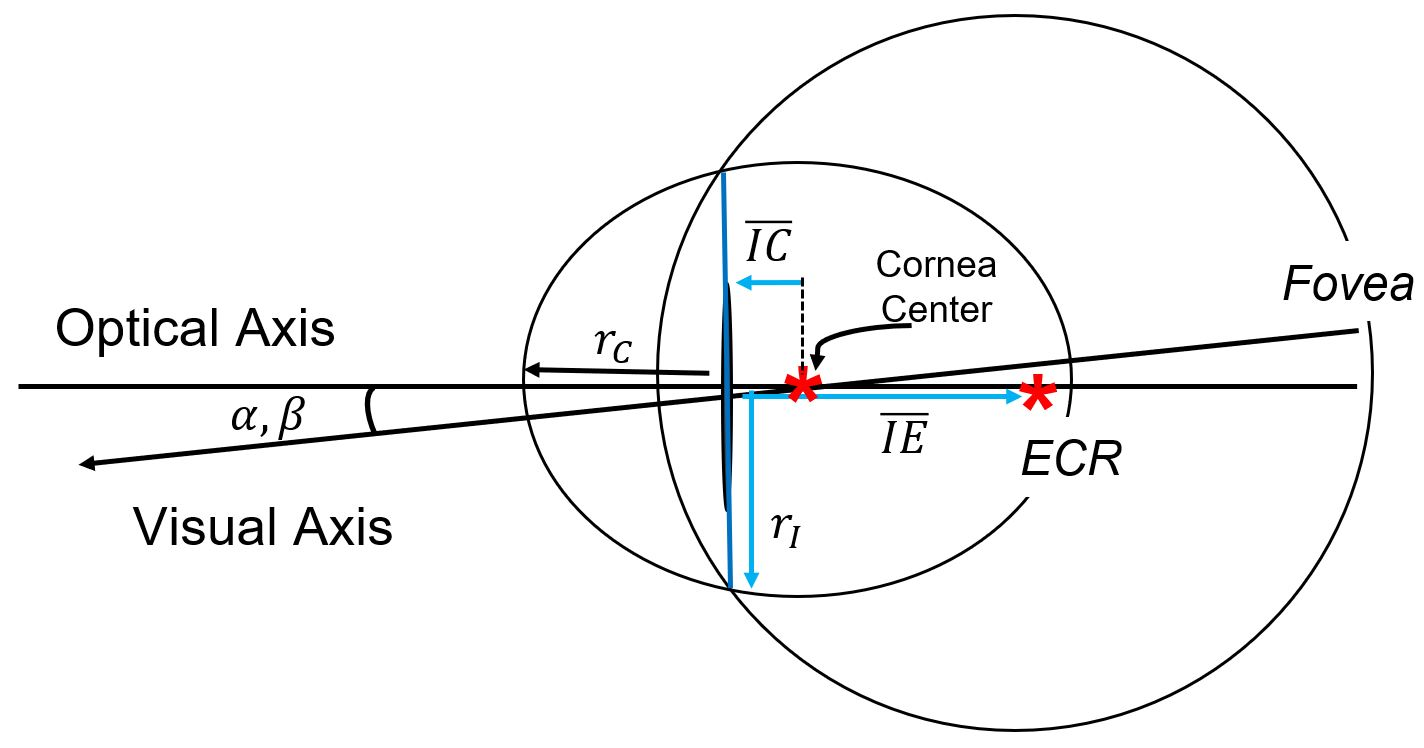
\includegraphics[scale=0.3]{./Pics/blink_eye_model}
    \caption{The proposed eye model.  The parameters' meaning are listed in Table \ref{tab:model_parameters}}
    \label{fig:model_drawing}
\end{figure}
%%%%%%%%%%%%%%%%%%%%%%%%%%%%%%%%%%%%%%%%%%%%%%%%%


The cornea is modelled as an ellipsoid with its center located on the line, at on offset $\bar{IC}$, that is parallel to the normal of the iris plane and which passes through the center of the circular iris and the eyeball center. The distance from the center of the iris to $ECR$ is denoted as $\bar{IE}$.  Similar to \cite{DierkesEtAl2018}, it is assumed that the cornea and the aqueous humor form a homogeneous medium with an effective refractive index n=1.33 \citep{GuestrinEizenman2006}.  We furthermore assume that the intersection of the cornea with the iris plane is the iris-sclera boundary.  Therefore, given the cornea center and the iris radius, two of the cornea's radii are equal and can be computed. The only free parameter is the major axis of the cornea denoted as $r_C$. Although, in reality, the cornea also encompass the iris, we assume that the projection of the limbus onto the camera plane is not affected by the refraction capabilities of the cornea.  

The pupil is assumed to lie on the iris plane.  Unlike \cite{DierkesEtAl2018}, we do not assume that the pupil is circular in shape nor that its center is aligned with that of the iris.  

The line connecting the cornea center and the iris center is the optical axis. The optical axis is the geometrical symmetry axis of the eye system.  The visual axis is defined by the line connecting the fovea and the cornea center, which deviates from the optical axis \citep{YoungSheena1975, Gross2008}.  The fovea is a region in the eye that allows highest visual acuity and it is this region onto which a user's area of interest is mapped to.  If the unit length vector $\textbf{N}_o$, denoting the optical axis in the eye camera coordinate system, is expressed as a function of two angles, $\phi$ and $\gamma$ as
\begin{equation}
    \textbf{N}_o =  \begin{bmatrix}
    \cos{(\phi)} \sin{(\gamma)}\\
    \sin{(\phi)}\\
    -\cos{(\phi)} \cos{(\gamma)}
  \end{bmatrix},
\end{equation}
then, by adding the angular terms $\alpha$ and $\beta$, we obtain the visual axis $\textbf{N}_v$:
\begin{equation}
    \textbf{N}_v =  \begin{bmatrix}
    \cos{(\phi + \alpha)} \sin{(\gamma + \beta)}\\
    \sin{(\phi + \alpha)}\\
    -\cos{(\phi + \alpha)} \cos{(\gamma + \beta)}
  \end{bmatrix} .
\end{equation}

Note that since the pupil's center may not necessarily coincide with the that of the iris \citep{Gross2008}, the optical axis is not necessarily the unit vector that lies on the line that connects the the centre of the entrance pupil and the cornea center. Let us denote the unit vector that connects the pupil center and the cornea center as $\textbf{N}_I$, which will make use of in the next section.


\subsection{Geometrically-based 2D iris contour fitting}
 The objective of the iris contour fitting task is to find the position of the model's eyeball center of rotation $ECR$ and $\bar{IE}$, given $r_I$, in the eye camera coordinate system such that the perspective projection of the model's limbus onto the camera's image plane will match the observed 2D limbus contour. Since we assume a full perspective projection under a pinhole camera model, the circular iris contour projects to an ellipse onto the image plane. This optimization problem is described in Algorithm \ref{alg:2d_iris_fitting}, where $\mathcal{R}_i(\textbf{N}_o| \xi, \eta)$ is the rotation matrix applied to $\textbf{N}_I$ (and the entire eye model) given the azimuthal and polar angles $\xi$ and $\eta$, respectively, for the $i$-th frame; $\mathcal{P}(\cdot)$ is the projection of the 3D iris onto the image plane, which results in an ellipse; $LP_{i,j}$ are the 2D coordinates of the $j$-th observed limbus points out of total $J_i$ points on the  $i$-th captured frame; and $\mathcal{D}(\cdot, \cdot)$ is a function that computes the euclidean distance of a point from an ellipse's contour. 

Let us reiterate that the optimization for $x,y,z,$ and $\bar{IE}$ is independent on the true gazing direction of the user.  Hence, if the eye model parameters listed in Table \ref{tab:model_parameters} have been optimized for a specific user at a given session, one can reoptimize only for $x,y,z,$ and $\bar{IE}$ as a new gaze inference session begins.

In the next section we describe how we utilize known points of interest focused on by the user to optimize $r_I$, and subsequently $\hat{x}, \hat{y}, \hat{z}$ and $\hat{\bar{IE}}$, and the other eye parameters for gaze prediction purposes.

\begin{algorithm}
    \caption{Geometrically-based 2D iris contour fitting Algorithm}
\begin{algorithmic}
    \REQUIRE (a) $N$ eye region frames of a user recorded by a camera; \\
    \STATE (b) Intrinsic parameters of the camera.\\
    \STATE (c) 2D limbus landmarks on image.\\
    \STATE (d) $r_I = 6$ mm \citep{Gross2008}.\\
    \RETURN {$\hat{x}, \hat{y}, \hat{z}, \hat{\bar{IE}}$}
    \STATE \textbf{Initialization}: Initial guess for $x,y,$ and $z$ obtained from the method proposed by \cite{SwirskiDodgson2013}. $\hat{\bar{IE}} = 12$ mm as initial guess \citep{Gross2008} .
    \WHILE{\textit{not converged}} 
    \FOR{$i=1...N$}
       \STATE {$\hat{\xi}_i, \hat{\eta}_i = \arg \min_{\xi, \eta} \sum_{j=1}^{J_i} \biggl|\biggl|\mathcal{D}(LP_{i,j}, \mathcal{P}(\mathcal{R}_i(\textbf{N}_I| \xi, \eta; x, y, z, \bar{IE}, r_I)))\biggr|\biggr|_2^2$} 
    \ENDFOR
       \STATE $\hat{x}, \hat{y}, \hat{z}, \hat{\bar{IE}} = \arg \min_{x,y,z,\bar{IE}} \sum_{i=1}^{N}\biggl|\biggl| \biggl[ \sum_{j=1}^{J_i} \mathcal{D}(LP_{i,j}, \mathcal{P}(\mathcal{R}_i(\textbf{N}_I| x, y, z, \bar{IE}; \hat{\xi}_i, \hat{\eta}_i, r_I))) \biggr] \biggr|\biggr|_2^2$
    \ENDWHILE
\end{algorithmic}
\label{alg:2d_iris_fitting}
\end{algorithm}
 

\subsection{Gaze Vector in LC and RC CS} 

At this stage, we let the remaining eye parameters listed in Table \ref{tab:model_parameters} to be defined as population average values. Now, once $\hat{x}, \hat{y}, \hat{z}, \hat{\bar{IE}}$ in the eye camera coordinate system are found, the angles $\hat{\xi}$ and $\hat{\eta}$ are computed for each captured eye frame given $LP$ using the first loss function defined in Algorithm \ref{alg:2d_iris_fitting}.  Then, upon rotating the eye model by $\hat{\xi}$ and $\hat{\eta}$, we unprojected the $M$ pupil landmarks in the $i$-th recorded frame from the image plane,  through the cornea surface, and onto the iris plane  by an inverse ray-tracing approach. 

Let us denote the 2D pupil landmarks points in pixels as $PL_{i,m}$, where $m=1,...,M$. The unprojection operation is carried out by first obtaining the 3D ray $\hat{e}_{i,m}$ along which the $PL_{i,m} = [x_{PL}, y_{PL}]_{i,k}^T$ landmark is located. To obtain $\hat{e}_{i,m}$ we first multiplied $PL_{i,m}$ by the inverse camera matrix $K$ to obtain ${e}_{i,m}$,
\begin{equation}
{e}_{i,m} = K^{-1} 
\begin{bmatrix}
x_{PL}\\
y_{PL}\\
1\\
\end{bmatrix}_{i,k}.
\end{equation}
Then, we normalized  ${e}_{i,m}$ to compute $\hat{e}_{i,m}$,
\begin{equation}
\hat{e}_{i,m} = {e}_{i,m} / ||{e}_{i,m}||_2.
\end{equation}

The $\hat{e}_{i,m}$ unit vector originates from the camera's origin and intersects the ellipsoidal cornea surface at $\rho_{i,m}$. At $\rho_{i,m}$, the ray along $\hat{e}_{i,m}$ undergoes refraction.  The refracted ray, $\hat{e}_{i,m}^{ref}$, intersects the iris plane and marks a location in 3D on the pupil boundary in the camera CS.  $\hat{e}_{i,m}^{ref}$ is defined as:
\begin{equation}
\hat{e}_{i,m}^{ref} =\eta \hat{e}_{i,m} + \biggl(\eta \left<\hat{e}_{i,m}, \hat{n} \right> - \sqrt{1 - \eta^2(1 - \left<\hat{e}_{i,m}, \hat{n} \right>^2)} \biggr)
\end{equation}
where $\eta = n_{\text{cornea}}/n_{\text{air}}$ and $\left<\textbf{a}, \textbf{b} \right>$ is the dot product of $\textbf{a}$ and $\textbf{b}$.

Once all $M$ have been unprojected onto the iris plane, their mean is taken as the pupil center. The unit vector of line connecting the center of the unprojected pupil on the iris plane and the cornea center is then regarded as the gaze vector, $N_o = N_v$, with $\alpha, \beta = 0$.
 

\subsection{Gaze Calibration Process}
In this section we describe the calibration and optimization process undertaken for the problem of gaze prediction.  Recall that each subject was asked to wear the HMD and be seated in front and at the center of the display unit at a distance of 0.8 meters. During the calibration step, the user is asked to look at 25 points shown to the user on the screen and located on top of a digital checkerboard pattern (Figure \ref{fig:pattern_monitor}).  

In order to be able to perform the optimization step for the eye model parameters, we needed to have the computed visual axis vectors of both eyes in the same CS as those of the point-of-interest markers. Therefore, at first, we estimated the locations of the markers in the world camera CS. The location, in pixels, of each of the 25 points on the screen is known as well as the size, in pixels, of the checkerboard pattern. We have measured the height and width of the display unit in mm such that the locations of the markers and checker sizes in the M CS can be computed.  Now, as the user was focusing his/hers attention on each of the markers, the screen was completely visible to the world camera.  Since the markers were displayed on top of a checkerboard pattern of known size, the screen plane as well as the location of the markers in 3D W CS were estimated using OpenCV's functions.

Next, the gaze vectors computed in the left and right eye camera CS were transformed to the world camera CS using the homogeneous transformation matrices $H^{LC}_W$ and $H^{RC}_W$, respectively.

The gaze vectors and the points of interest $POR$ in the world camera CS were input to an optimization process that aims to estimate the set of eye parameters that minimizes the following loss function:
\begin{equation} \label{eq:por_loss}
\hat{\theta} = \\
\arg \min_{\theta} \sum_{l=1}^{L} ||\hat{POR}_l(\bar{IC}, r_C, n_{\text{cornea}}, \alpha, \beta; \hat{x}, \hat{y}, \hat{z}, \hat{\bar{IE}}, r_I) - POR_l||_2^2,
\end{equation}
where $\theta = \{\bar{IC}, r_C, n_{\text{cornea}}, \alpha, \beta \}$, $l=1,...,L$ are the frames that correspond to the user focusing at specific points of interest; and $\hat{POR}_l$ is the mean predicted point of interest by both eye models in the world CS on the screen plane.  

Since, the initially assumed $r_I$ will affect the computed loss in Equation \ref{eq:por_loss}, it is beneficial to optimize for $r_I$ as well. The complete algorithm used for optimizing all of the eye model parameters listed in Table \ref{tab:model_parameters} is shown in Algorithm \ref{alg:eye_param_optim}.

\begin{algorithm}
    \caption{Optimization Algorithm for the Eye Model Parameters}
\begin{algorithmic}
    \REQUIRE (a) $L$ eye region frames of a user recorded by a camera with corresponding points of interests $POR$; \\
    \STATE (b) Intrinsic parameters of the camera.\\
    \STATE (c) 2D limbus landmarks on images.\\
    \RETURN {$\hat{x}, \hat{y}, \hat{z}, \hat{\bar{IE}}, r_I, \bar{IC}, r_C, n_{\text{cornea}}, \alpha, \beta$}
    \STATE \textbf{Initialization}: $\hat{x}, \hat{y}, \hat{z}, \hat{\bar{IE}}$ obtained from Algorithm \ref{alg:2d_iris_fitting}.
    \FOR{$r_I \in [5.5, 6.5]$}
       \STATE {Estimate $\hat{x}, \hat{y}, \hat{z}$, and $\hat{\bar{IE}}$ using Algorithm \ref{alg:2d_iris_fitting}. The initialization for  Algorithm \ref{alg:2d_iris_fitting} are the previous iteration's $\hat{x}, \hat{y}, \hat{z}$, and $\hat{\bar{IE}}$.} 
       \STATE {$\hat{\theta} = \arg \min_{\theta} \sum_{l=1}^{L} ||\hat{POR}_l(\bar{IC}, r_C, n_{\text{cornea}}, \alpha, \beta; \hat{x}, \hat{y}, \hat{z}, \hat{\bar{IE}}, r_I) - POR_l||_2^2$}
    \ENDFOR
    \STATE Select $\hat{x}, \hat{y}, \hat{z}, \hat{\bar{IE}}$, and $\hat{\theta}$ which produces lowest loss in:
    \STATE {$\sum_{l=1}^{L} ||\hat{POR}_l(r_I, \hat{x}, \hat{y}, \hat{z}, \hat{\bar{IE}}\bar{IC}, r_C, n_{\text{cornea}}, \alpha, \beta) - POR_l||_2^2$}
    
\end{algorithmic}
\label{alg:eye_param_optim}
\end{algorithm}

\section{Results}
\subsection{Eye camera - World camera calibration}

\subsection{Iris fitting}
Figure \ref{fig:iris_fitting} depicts the pupil and iris fitting for User 1 based on located limbus points and the optimization procedure as stated in Algorithm \ref{alg:2d_iris_fitting}. Correctly estimating the center of rotation of the eye model allows to fit limbus contours even at large angular eye movements.  Thus, allowing our model to estimate the gaze direction of a user at such extreme angles. 

%%%%%%%%%%%%%%%%%%%%%%%%%%%%%%%%%%%%%%%%%%%%%%%%%
\begin{figure}[h!]
    \center
    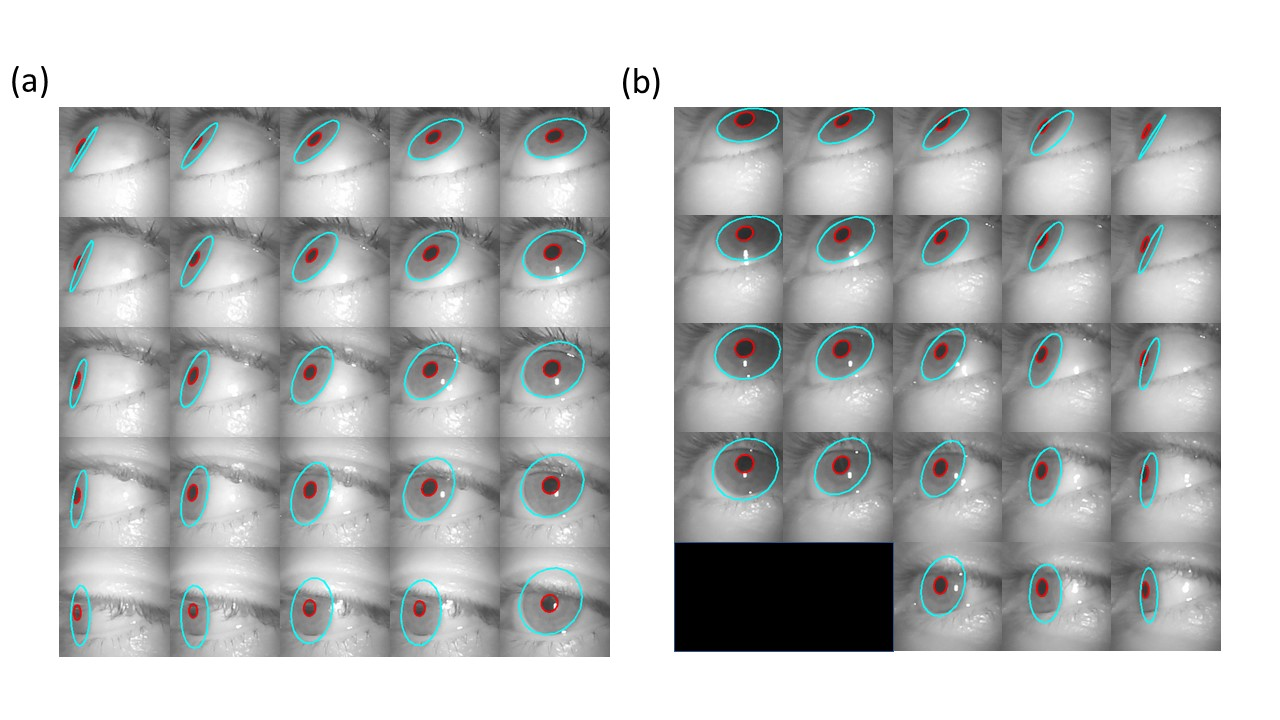
\includegraphics[scale=0.4]{./Pics/iris_fitting.JPG}
    \caption{Iris fitting (magenta) and pupil fitting (red) results based on located limbus points and the optimization procedure as stated in Algorithm \ref{alg:2d_iris_fitting}. (a) Left eye camera  and (b) right eye camera located on the glasses. At each frame the user is looking at a different marker on the screen. The missing images in black are images that were not recorded during the experiment. } 
    \label{fig:iris_fitting}
\end{figure}
%%%%%%%%%%%%%%%%%%%%%%%%%%%%%%%%%%%%%%%%%%%%%%%%%

\subsection{Gaze estimation analysis}
\subsubsection{Sensitivity to limbus localization method}
The algorithm for limbus localization is partly based on a machine learning solution. Its robustness is crucial for the correctly estimating user's gaze direction.  To analyze the effects of the limbus prediction method on the estimated gaze, we have noted the standard deviation in the azimuthal and polar gaze angles $\xi$ and $\eta$ for the time spent by the user gazing at each of the 25 marker points.  These results are presented in Tables \ref{tab:std_limbus_gaze_error_cam_left} and \ref{tab:std_limbus_gaze_error_cam_right}. We note for non-extreme gaze angles, the standard deviation of the polar gaze angles are less than 0.1 degrees.


%%%%%%%%%%%%%%%%%%%%%%%%%%%%%%%%%%%%%%%%%%%%%%%%%
\begin{table}[h!]
\caption{Standard deviations of the gaze angles ($\xi$, $\eta$) in degrees due to predicted limbus points for each of the 25 markers presented to the user for the left eye camera.  }
\vspace{0.5cm}
\centering
\begin{tabular}{|l|c|c|c|c|c|c|c|c|c|c|}
\hline
& \multicolumn{5}{|c|}{Column} \\
\hline
\multirow{5}{*}{Row} & 0.078, 0.101  & 0.050, 0.019 & 0.219, 0.046 & 0.024, 0.033 & 0.021, 0.040 \\ \cline{2-6}
                & 0.083, 0.140 & 0.118, 0.033  & 0.029,0.030  & 0.023, 0.028 & 0.024, 0.043 \\  \cline{2-6}
                & 0.161, 0.152 & 0.210, 0.033 & 0.031, 0.025 & 0.026, 0.035 & 0.026, 0.048 \\  \cline{2-6}
                & 0.099, 0.147 & 0.032, 0.020 & 0.028, 0.025 & 0.026, 0.035 & 0.028, 0.064 \\  \cline{2-6}
                & 0.098, 0.140 & 0.025, 0.019   & 0.033, 0.031   & 0.006, 0.027  & 0.033, 0.098  \\ 
\hline
\end{tabular}
\label{tab:std_limbus_gaze_error_cam_left}
\end{table}

\begin{table}[h!]
\caption{Same as Table \ref{tab:std_limbus_gaze_error_cam_left} only for the right eye camera.  }
\vspace{0.5cm}
\centering
\begin{tabular}{|l|c|c|c|c|c|c|c|c|c|c|}
\hline
& \multicolumn{5}{|c|}{Column} \\
\hline
\multirow{5}{*}{Row} & 0.135,0.115 0  & 0.050,0.043  & 0.219, 0.039 & 0.024, 0.025 & 0.021, 0.024 \\ \cline{2-6}
                & 0.131, 0.120 & 0.025, 0.055 & 0.031,0.033  & 0.028,0.034  & 0.029, 0.019 \\  \cline{2-6}
                & 0.141, 0.113 & 0.028, 0.058 & 0.040,0.037  & 0.018,0.039  & 0.032, 0.021 \\  \cline{2-6}
                & 0.145, 0.085  & 0.046, 0.118 & 0.052, 0.025  & 0.022,0.042  & 0.036,0.024  \\  \cline{2-6}
                & 0.014, 0.018 & 0.039, 0.110   & 0.061, 0.023   & 0.029, 0.044 & 0.039, 0.020 \\ 
\hline
\end{tabular}
\label{tab:std_limbus_gaze_error_cam_right}
\end{table}
%%%%%%%%%%%%%%%%%%%%%%%%%%%%%%%%%%%%%%%%%%%%%%%%%

\subsubsection{Gaze angles angular difference between markers}
       

\section{Discussion}
\subsection{Usability of Naneye cameras}
Although this report was mainly focued on IR-based camera settings, the presented algorithms and methods can also be applied to webcam-type settings which utilize RGB cameras.  However, one does need to have an algorithm for locating iris and pupil contours in such settings. In our case, Blink's contour detection algorithm can also be applied. An example which showcases Blink's contour detection capabilities is presented in Figure \ref{fig:naneye}b. In this example, a user is wearing a head set with Naneye cameras placed at four different locations on the rim of the glasses Figure \ref{fig:naneye}a. The cameras' parameters are listed in table \ref{tab:spec}. 

%%%%%%%%%%%%%%%%%%%%%%%%%%%%%%%%%%%%%%%%%%%%%%%%%
\begin{figure}[h!]
    \center
    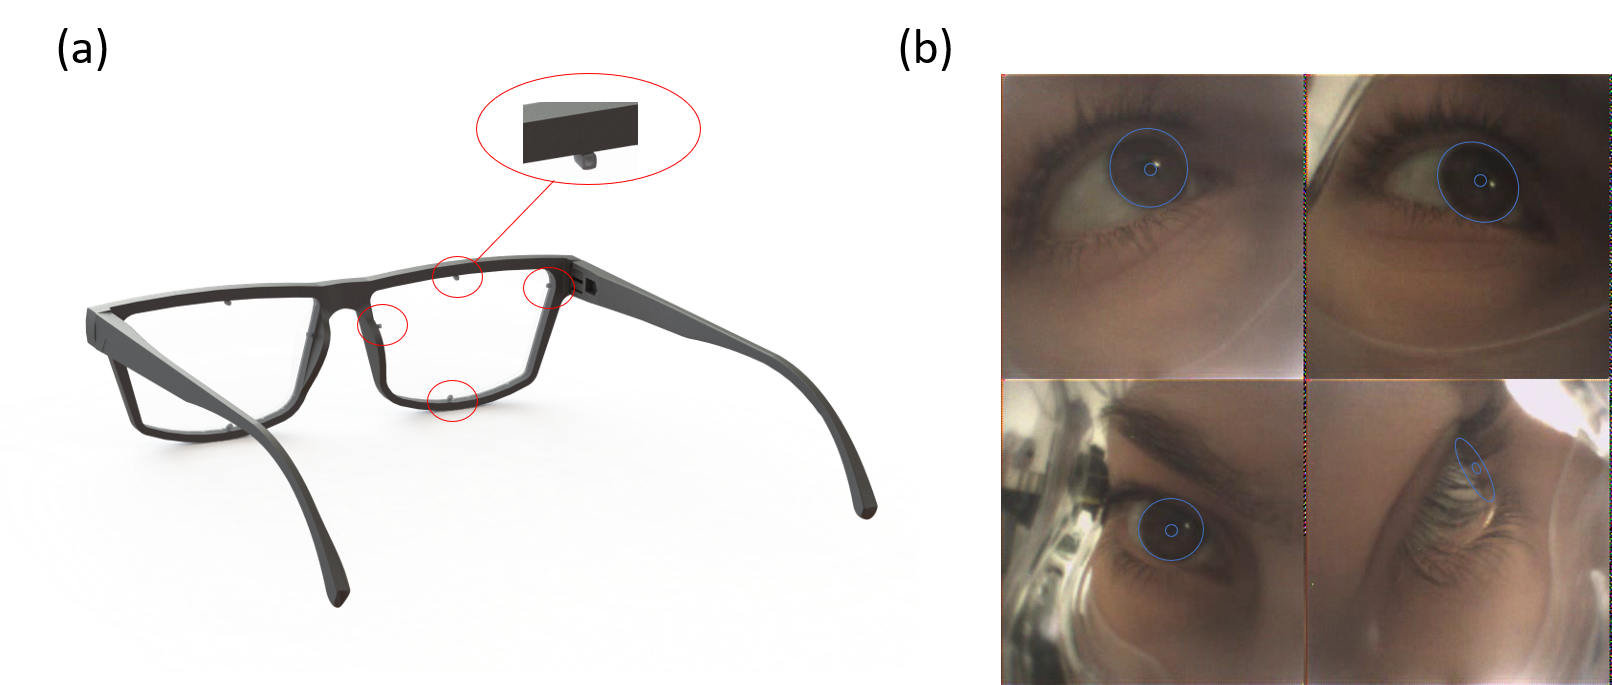
\includegraphics[scale=0.4]{./Pics/naneye2.png}
    \caption{(a) Location of four Naneye cameras mounts on the glasses. (b) Images of the eye from the wearable device. In each image, pupil and iris contours are shown as estimated by Blink's algorithm.} 
    \label{fig:naneye}
\end{figure}
%%%%%%%%%%%%%%%%%%%%%%%%%%%%%%%%%%%%%%%%%%%%%%%%%
 
%%%%%%%%%%%%%%%%%%%%%%%%%%%%%%%%%%%%%%%%%%%%%%%%%
\begin{figure}[h!]
    \center
    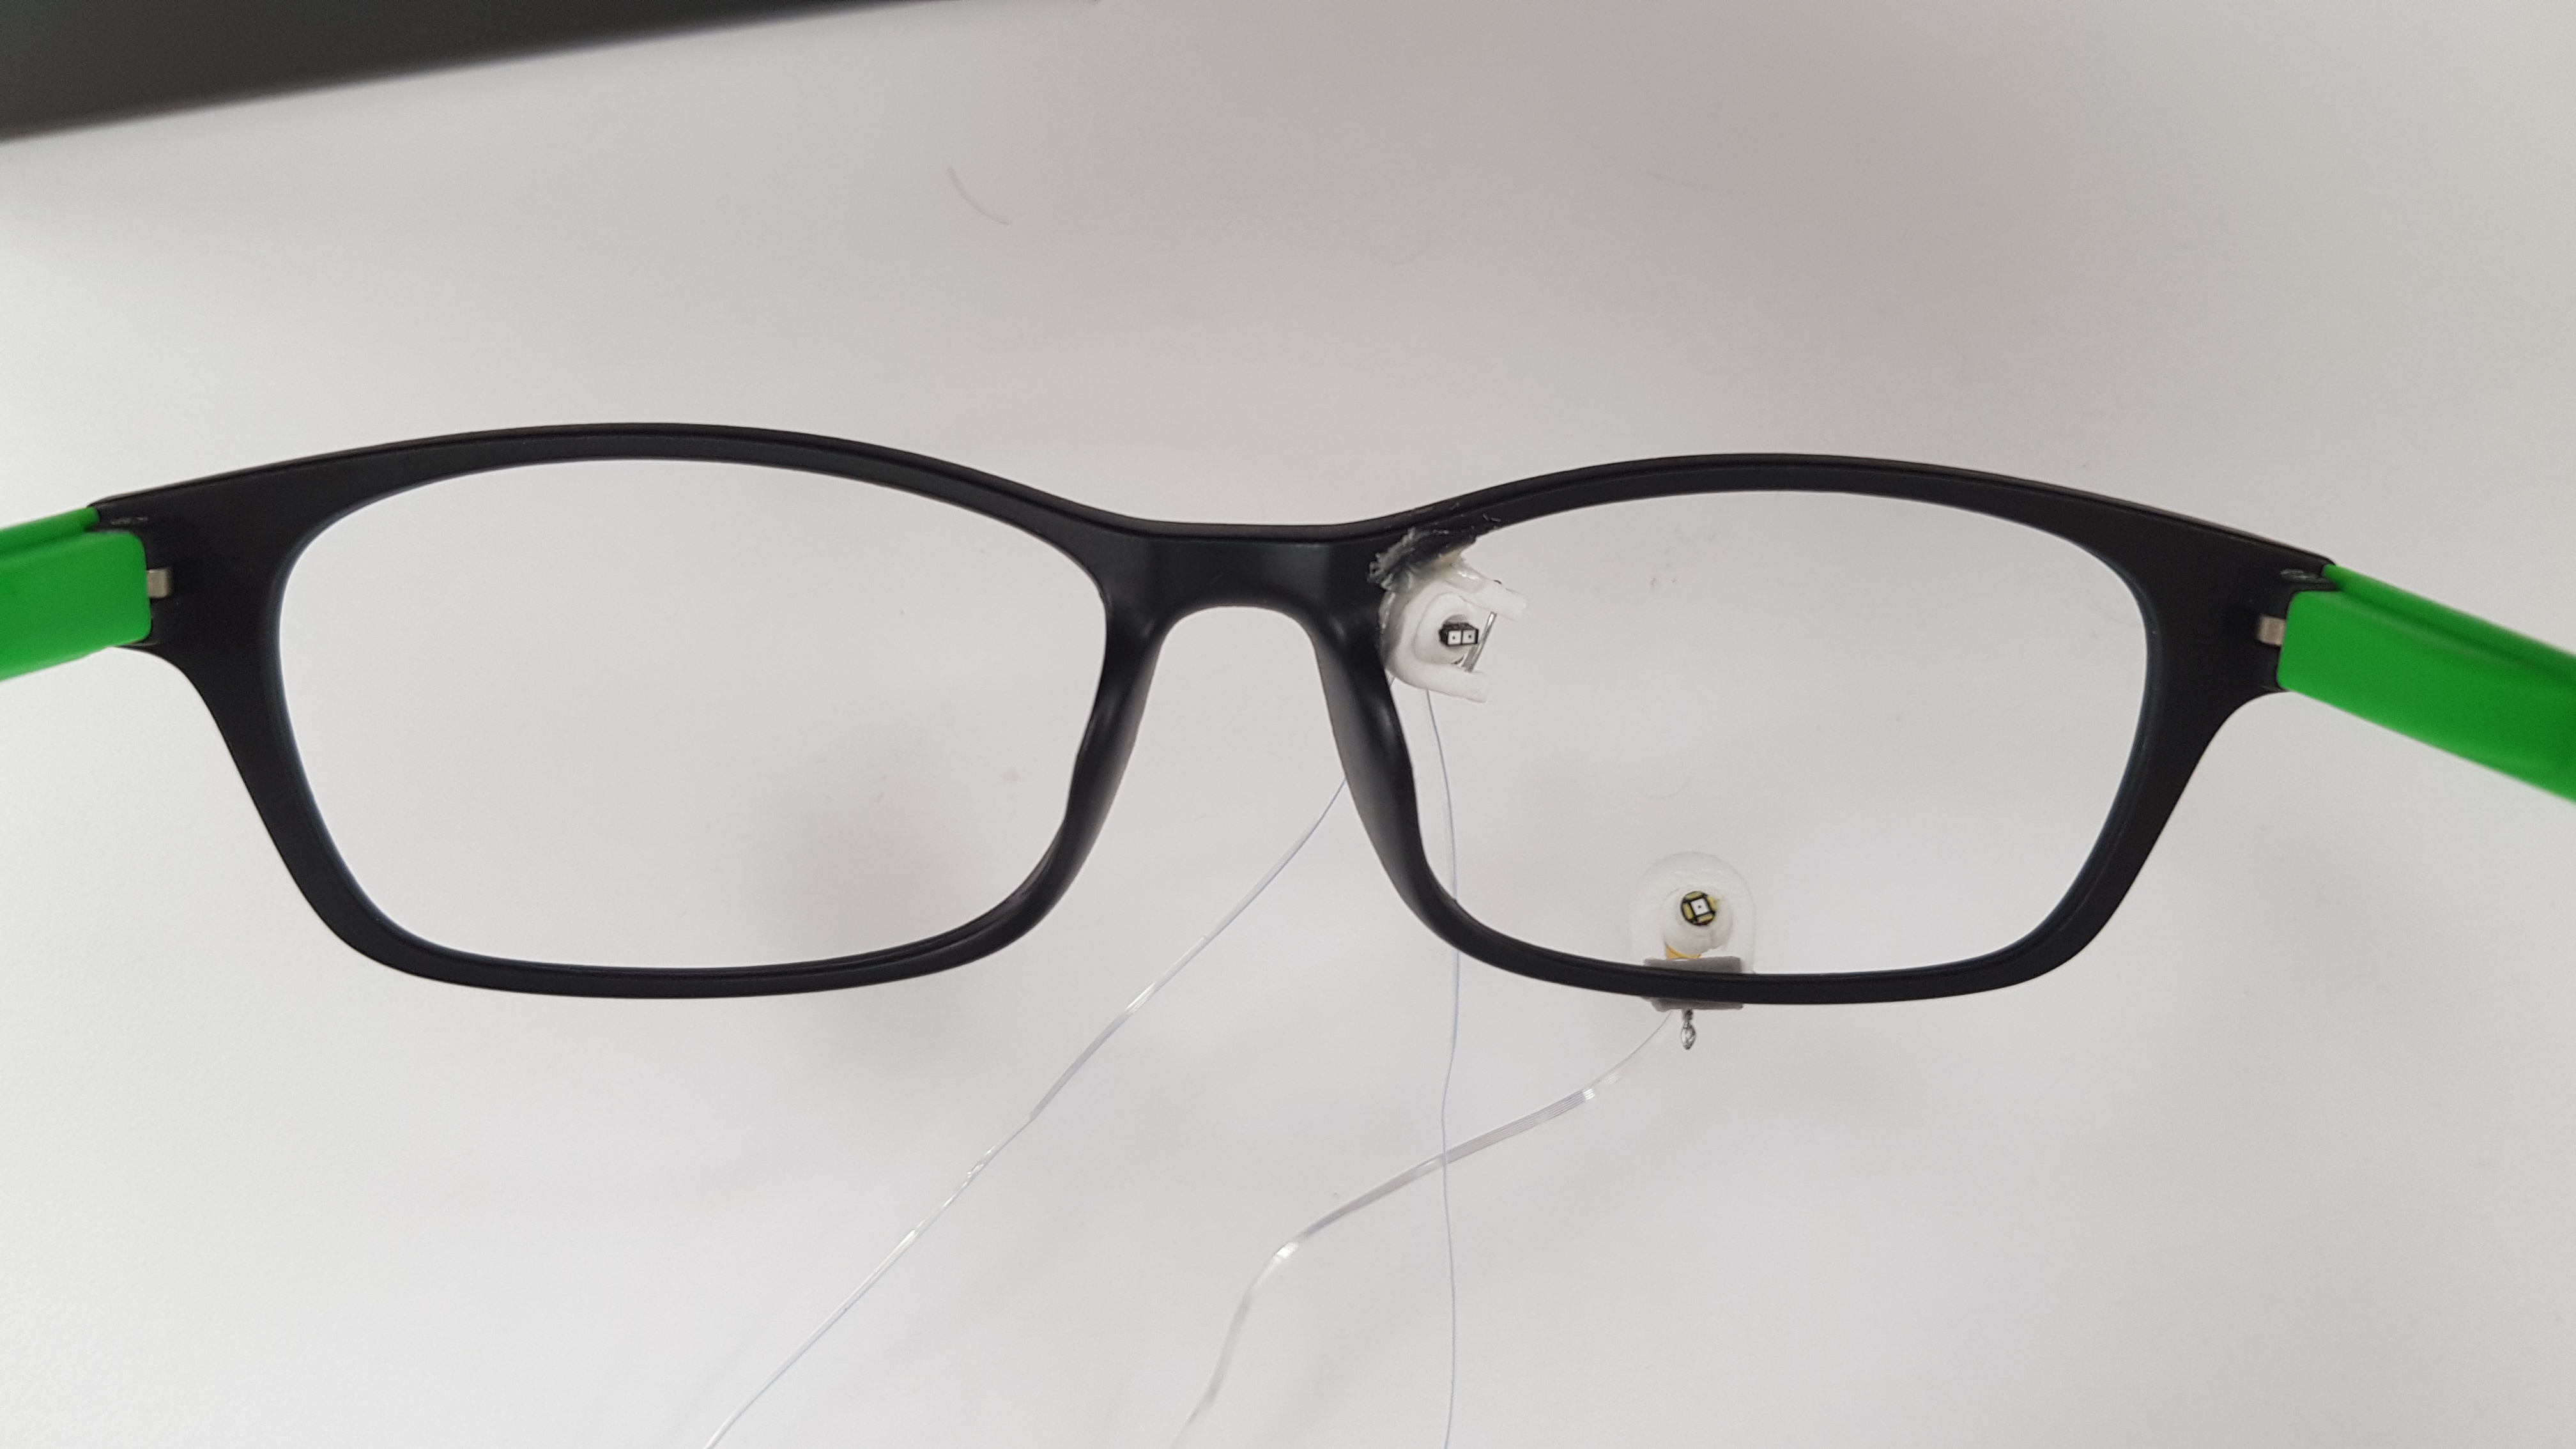
\includegraphics[scale=0.1]{./Pics/real_glasses_with_naneye.jpg}
    \caption{Two cameras placed on the glasses} 
    \label{fig:naneye2}
\end{figure}
%%%%%%%%%%%%%%%%%%%%%%%%%%%%%%%%%%%%%%%%%%%%%%%%% 
\begin{table}
\centering
\caption{\label{tab:spec} Specification NanEye image sensor}
\vspace{0.5cm}
\resizebox{0.7\textwidth}{!}{
\begin{tabular}{|c|c|c|}
\hline
Parameter & Value & Remark \\ \hline
Number of Pixels & $62.5$k, $250 \times 250$ &  \\ \hline
Pixelsize &  $3\mu m \times 3\mu m$ &\\ \hline
Color &  Bayer Pattern RGB &\\ \hline
Shutter & Rolling & \\ \hline
Dynamic range & 42dB & \\ \hline
Responsivity & 8DN/nJ/cm^2 & \\ \hline
Full well capacity & 10ke-  & \\ \hline
Temporal Noise dark rms  & $2$DN & \\ \hline
FPN & $<0.5\%$ & Corrected by Software  \\ \hline
PRNU & $<1\%$ & Corrected by Software  \\ \hline
Data output & 10bit digital LVDS & \\ \hline 
Supply & 1.8V &  \\ \hline
Framerate & 44fps & \\ \hline
Size & $1000 \mu m \times 1000 \mu m$ & $960 \mu m + 40 \mu m$ dicing  \\ \hline
Number of pads & 4 & VDD, VSS Data+, Data-  \\ \hline
\end{tabular}}
\end{table}
%4. Thae sphere eye-t are required to tracking rpised of erformance is expected to be displayed in angular error, target point-comparative, and subject-comparative way

%5. If you are possible, please records a demo video clip for helping us to understand your validation process

\bibliographystyle{plain}
\bibliography{references}
\end{document}
